\documentclass{article}[12 pt]

\usepackage[utf8]{inputenc}
\usepackage[english]{babel}
\usepackage{tocloft}
\usepackage{lipsum}
\usepackage{sidecap}


\renewcommand\cftsecfont{\normalfont}
\renewcommand\cftsecpagefont{\normalfont}
\renewcommand{\cftsecleader}{\cftdotfill{\cftsecdotsep}}
\renewcommand\cftsecdotsep{\cftdot}
\renewcommand\cftsubsecdotsep{\cftdot}

\usepackage{graphicx}
\usepackage{hyperref,xcolor}

\definecolor{wine-stain}{rgb}{0.5,0,0}

\hypersetup
{
    colorlinks=true,
    linktoc = all,
    linkcolor = wine-stain,
    urlcolor = blue
}

\begin {document}

\title{Math Graphics README}
\author{Frank Basile, Janice Wallace}
\maketitle

\tableofcontents
	\section{Introduction}
		Math Graphics is the final project for Group 12. The program is a fairly robust graphing calculator capable of displaying visual representations of mathematical functions on 2D Cartesian, 2D Polar, and 3D Cartesian graphs. Aside from displaying input functions, the calculator can also display derivatives and calculate definite integrals of single-variable functions in Cartesian 2D mode. Other features of the program include the ability to output the image of the graph to a file, as well as writing the independent and dependent variable data to a data format separated by any series of ASCII characters. Other features include the ability to customize the interface through the use of color changing palettes.

	\section{Installation}
	    No specific installation instructions are required. All that is required to run the program should be an updated version of Java and the executable file named MathGraphics.jar. For the latest version of Java, please check the \href{http://www.java.com}{Java homepage}.
	    
	\section{Starting the Program}
		Math Graphics has an easy to run interface. All that is required is to double click the MathGraphics.jar executable file. 
		
	\section{How To}
		\subsection{Initial Startup}
		When the program initially starts, the grapher is in Cartesian 2D mode and the function $sin(x)$ is displayed.:
			\begin{figure}[h!]
 				\centering
 				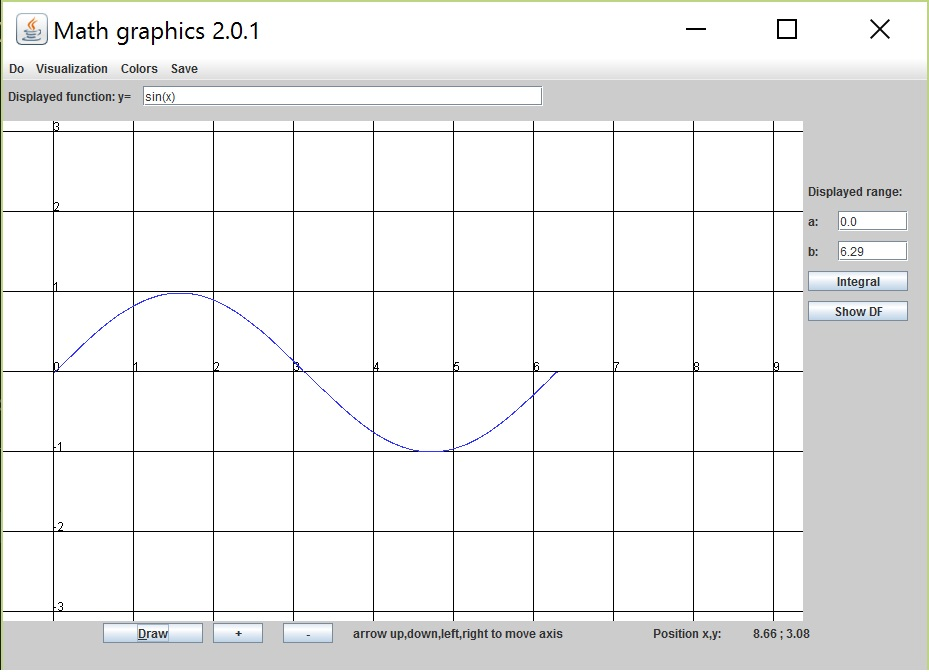
\includegraphics[scale = .80]{startupScreen}
 				\caption{The startup screen: $sin(x)$ is displayed}
 			\end{figure}

		\pagebreak
		\subsection{Basic 2D Cartesian Navigation}
		User interactions with the Math Grapher application take place by clicking on the appropriate buttons and menu bar items. The items in the 2D Cartesian window are shown in Figure 2.  Though Polar 2D is not shown, the layout is almost identical. 
			\begin{figure}[h!] 
				\centering
				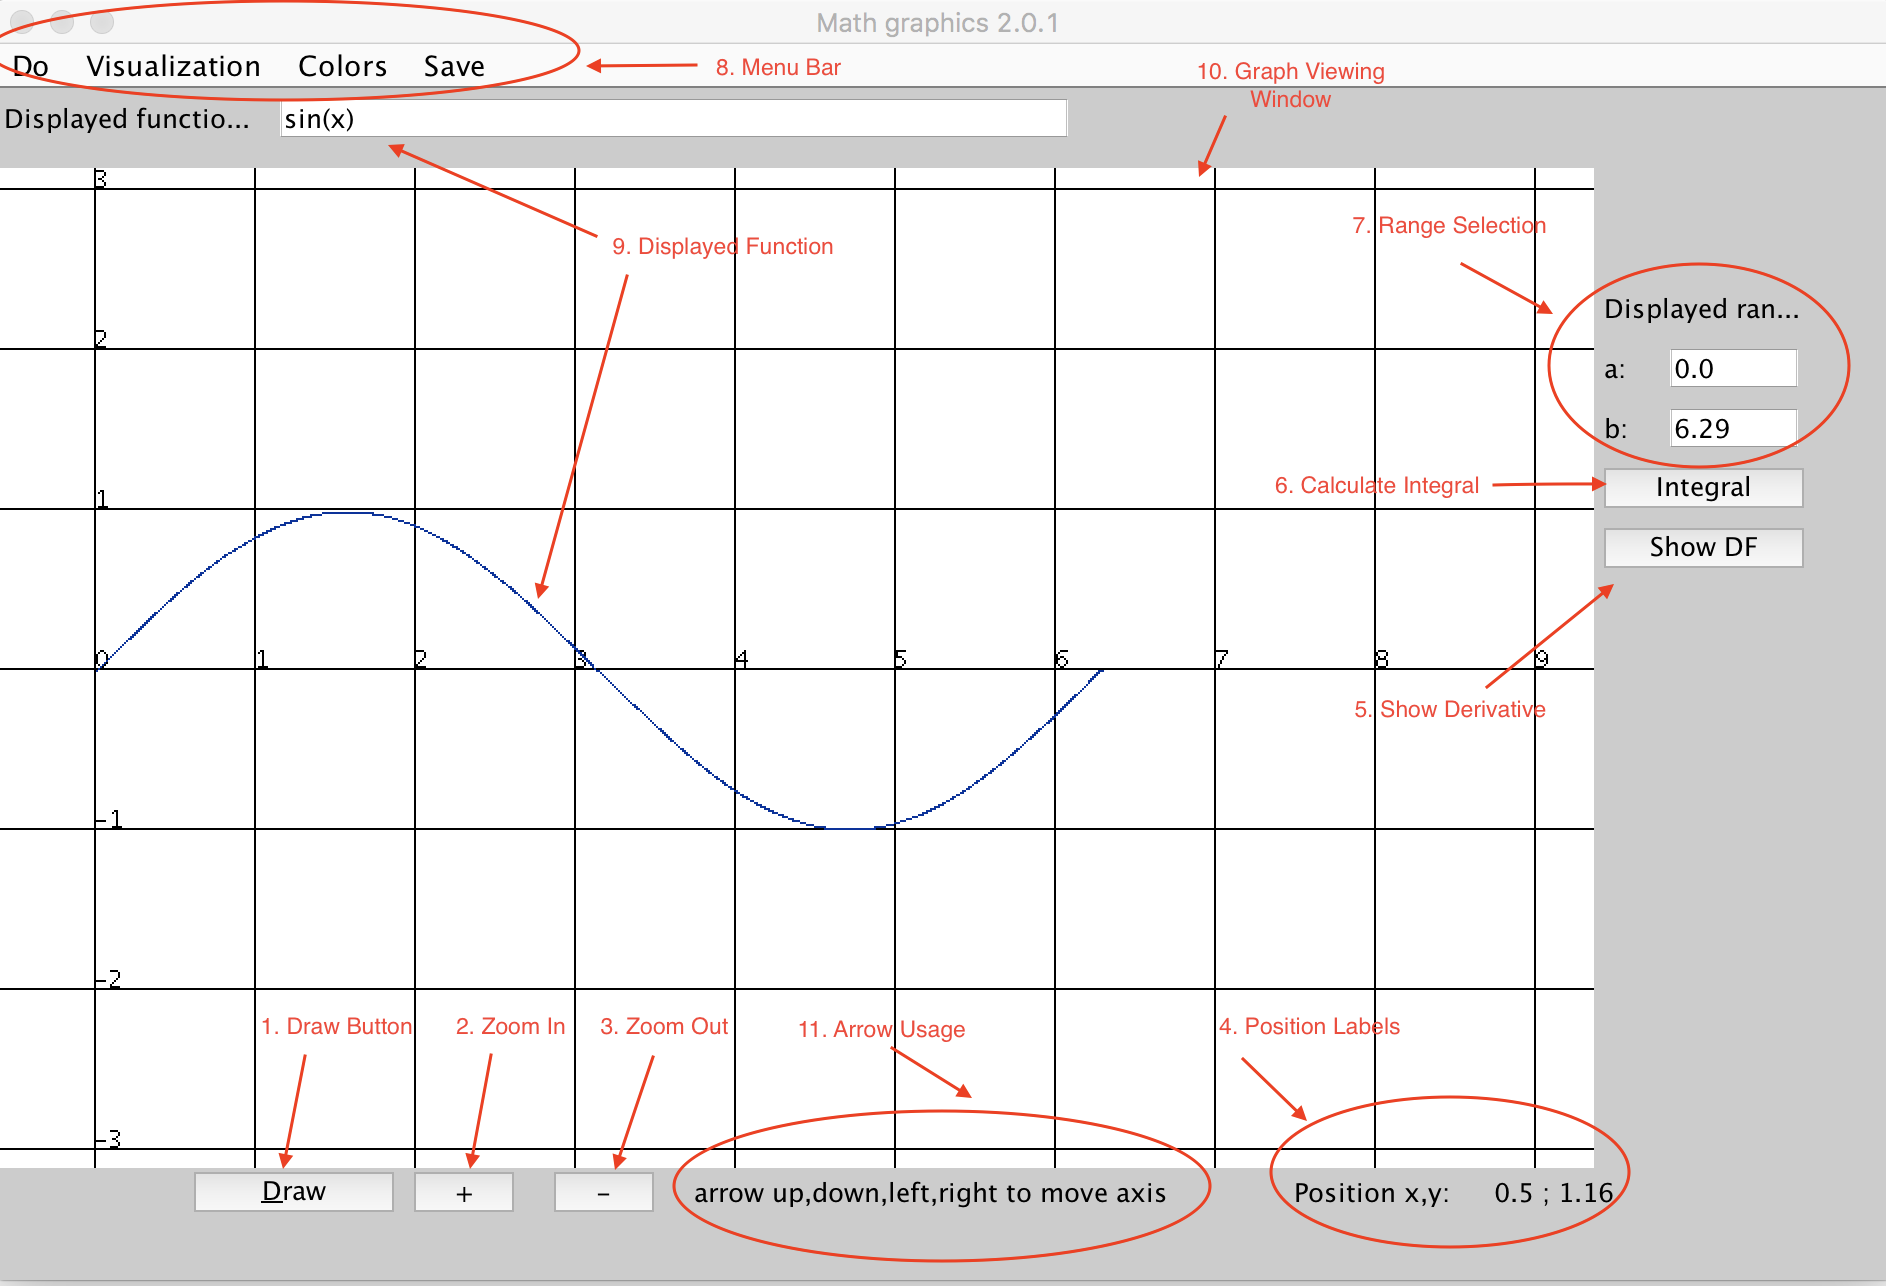
\includegraphics[scale = .30]{Map}
				\caption{Navigation items are labeled in red}
			\end{figure}
 		
			\subsubsection{Draw Button}
			The draw button (1) is used to paint the displayed function (9) into the graph viewing window (10). Any time the displayed function is changed, the draw button should be clicked. This will both validate the input and, if valid, draw the function. Alternatively, the menu bar (8) can be used by pressing ``Do" and then ``Draw" from the drop down menu.
 				
 			\subsubsection{Zoom In Function}
			The graph can be zoomed in to specific points by clicking the ``+'' button (2) located at the bottom of the screen. The graph will zoom in to the current center of the viewable graph. 
			
			\subsubsection{Zoom Out Function}
			The graph can be zoomed out of specific points by clicking the "-" button (3)  located at the bottom of the screen. The graph will zoom out from the center of the graph viewing window.
			
			\subsubsection{Position Labels}
			The position labels (4) serve as a reference point to the location on the graph viewing window (10) that the mouse pointer is currently hovering over. This can serve as an approximation to determining the input and output values of various functions.
 		
		 	\subsubsection{View the Graph of the Derivative}
 			The derivative can be displayed by pressing the ``Show DF'' button (5). Alternatively, the derivative can be displayed from the drop down menu (8) by clicking ``Do'' and ``Show DF.'' To hide the derivative simply press the ``No'' DF button (not shown). Or, from the drop down menu, select ``Do'' and ``No DF''.
 				\begin{figure}[h!]
 					\centering
 					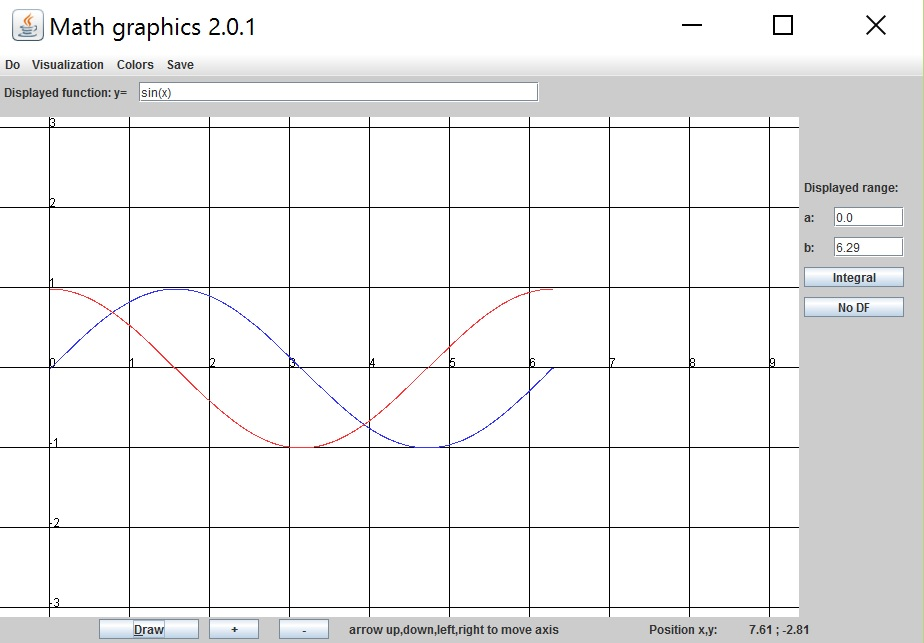
\includegraphics[scale = .75]{showDF}
					\caption{The derivative drawn after ``Show DF'' selected}
 				\end{figure}	
			
			\pagebreak
			\subsubsection{Integral Calculations}
			Definite integral calculations can be performed by pressing the ``Integral" button (6). After pressing the integral button, a new window will appear.
				\begin{figure}[h!]
					\centering
					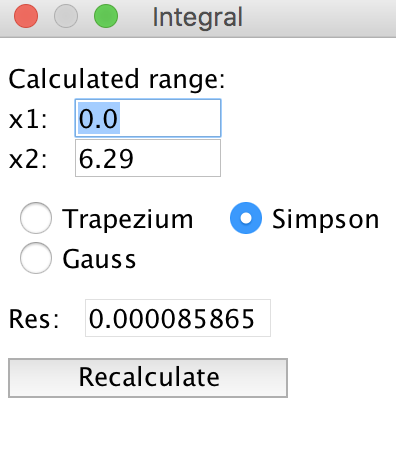
\includegraphics[scale=.5]{integral}
					\caption{Integral pop-up window}
				\end{figure}
				Once the integral window appears, the default range will be whatever range a and b were set to on the main display. The user has three integral calculations they can choose from: Simpson, Trapezium, and Gauss. Due to the way calculations are performed, there may be slight differences between the three - but usually no more than several thousandths. After a range is entered, and a selection made, the user will hit the recalculate button. In the result field, the newest calculation will appear.
				
			\subsubsection{Range Changes}
 			Range changes can be made to the displayed function. In order to do this, simply change the values of fields $a$ and $b$ (7). Only valid numeric values can be input to these fields. It is not a requirement that $a < b$ as both the function and derivative can be drawn with $a \leq b$ or $a \geq b$. After any changes are made, it is necessary to hit the ``Draw" button (1) or from the drop-down menu bar, select ``Do" and then ``Draw."
			
			\subsubsection{Menu Bar}
			The Menu Bar (8) provides the user with the ability to perform some of the same functions as the clickable buttons. The "Do" Menu allows the user to redraw the function, bring up the integral window, and show or hide the derivative of the displayed function. The ``Visualization" menu allows the user to view the graph in Cartesian 2D, Polar 2D or Cartesian 3D modes. The "Colors" menu gives the option for the user to change the color of the interface, and the ``Save" menu offers the opportunity to save the displayed image or export the data to a file. 
 	
			\subsubsection{Displayed Function}
			The Displayed Function (9) is perhaps one of the most important parts of the entire program. It is here where the user will enter functions to be calculated, and displayed in the graph viewing window (10). The engine behind the displayed functions can take in most single-variable functions including trigonometric functions. However, multiplication is not implicitly undertood. For example, common mathematical notation will use the form $ax$ to represent ``a times x.''Math Grapher requires that all multiplication is explicitly stated. Thus, $ax$ should be represented as ``a*x''. \\
			
			Another error some may make is not wrapping the variable of trigonometric functions in parentheses. Math Grapher requires that the variable be wrapped in parentheses such as: $sin(x)$ instead of $sinx$. If the displayed function is incorrectly entered, the user will receive a warning that there was an error parsing the function, and they are subsequently referred to this readme file.
			
			\subsubsection{Graph Viewing Window}
			The Graph Viewing Window (10) displays the input function entered in the ``Displayed Function'' field (9). In 2D mode, it houses an x and y axis in increments of 1. When the viewing windows is zoomed in, the increments are divided in half with each ``zoom in click'' and doubled with each ``zoom out click.''
			
			\subsubsection{Arrow Usage}
			The arrow keys can be used to scroll the graph viewing window (10) in the corresponding direction of the key value. 
			
	\subsection{Polar 2D Mode}
		One of the features of Math Grapher is the ability to view displayed functions in Cartesian 2D, Polar 2D, or Cartesian 3D modes. Despite the difference in modes, the basic use and interface remains the same as in Cartesian 2D mode. Thus, only the differences will be covered.

		\subsubsection{Entering Polar Mode}
			In order to enter Polar Mode, go to the drop down menu and select ``Visualizations.'' Then select ``Polar 2D.'' 
				\begin{figure}[h!]
					\centering
					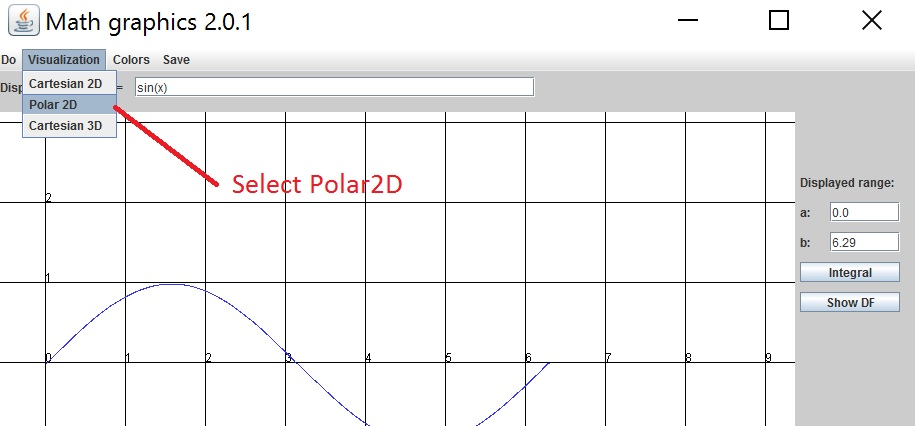
\includegraphics[scale = .75]{polar}
					\caption{Selecting Polar 2D mode from the menu bar}
				\end{figure}
				
			After Polar 2D mode is selected, the window will now be in Polar 2D mode. Notice that this view does not look much different from Cartesian 2D mode. In fact, there are only a few slight changes. The first change is that the example function, $sin(x)$ is now graphed on polar coordinates rather than Cartesian coordinates. The displayed function label has been changed to represent r(theta), and the range has also been changed to represent a range from ``Theta 1'' to ``Theta 2.'' Also removed are the abilities to calculate definite integrals and view the derivative of the functions.
				\begin{figure}[h!]
				\centering
				 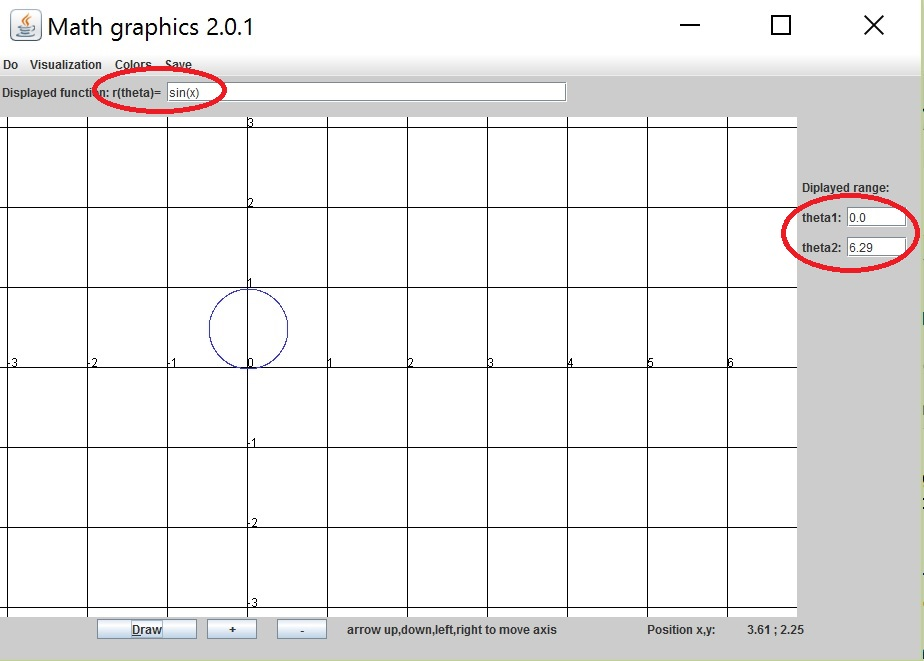
\includegraphics[scale=.70]{polarMode}
				 \caption{Changes in Polar 2D Mode circled in red. Notice that $sin(x)$ is graphed as a polar function}
				\end{figure}
				\pagebreak
	\subsection{Cartesian 3D Mode}
		Cartesian 3D Mode has the capability of viewing functions of two variables in a 3-Dimensional setting. Inputting functions into the "displayed function" field is the same as both 2D modes with one exception. Because the third dimension, $z$, is dependent on inputs to $x$ and $y$, all functions assume both $x$ and $y$ variables. In the case that $x$ or $y$ are not explicitly defined, such as the case of the function $x^2$ the function is implicitly defined as $x^2 + 0y$. 
	
		\subsubsection{Entering Cartesian 3D Mode}
		Entering Cartesian 3D mode is similar to entering either of the 2D modes. Simply go to the menu bar, click ``Visualizations," and then select ``Cartesian 3D," as shown in Figure 7.

		\subsubsection{3D Navigation}
		The graph viewing window in Cartesian 3D is slightly different in that the 2-Dimensional Grid is no longer present, and has been replaced by a 3-Dimensional axis. Also, the displayed ranges allow for range changes to both the $x$ and $y$ axis. Upon entering the 3D window, whatever function had been previously graphed in either Cartesian 2D or Polar 2D modes will be represented. In this case, we still use the $sin(x)$ function. 
			\begin{figure}[h!]
			\centering
			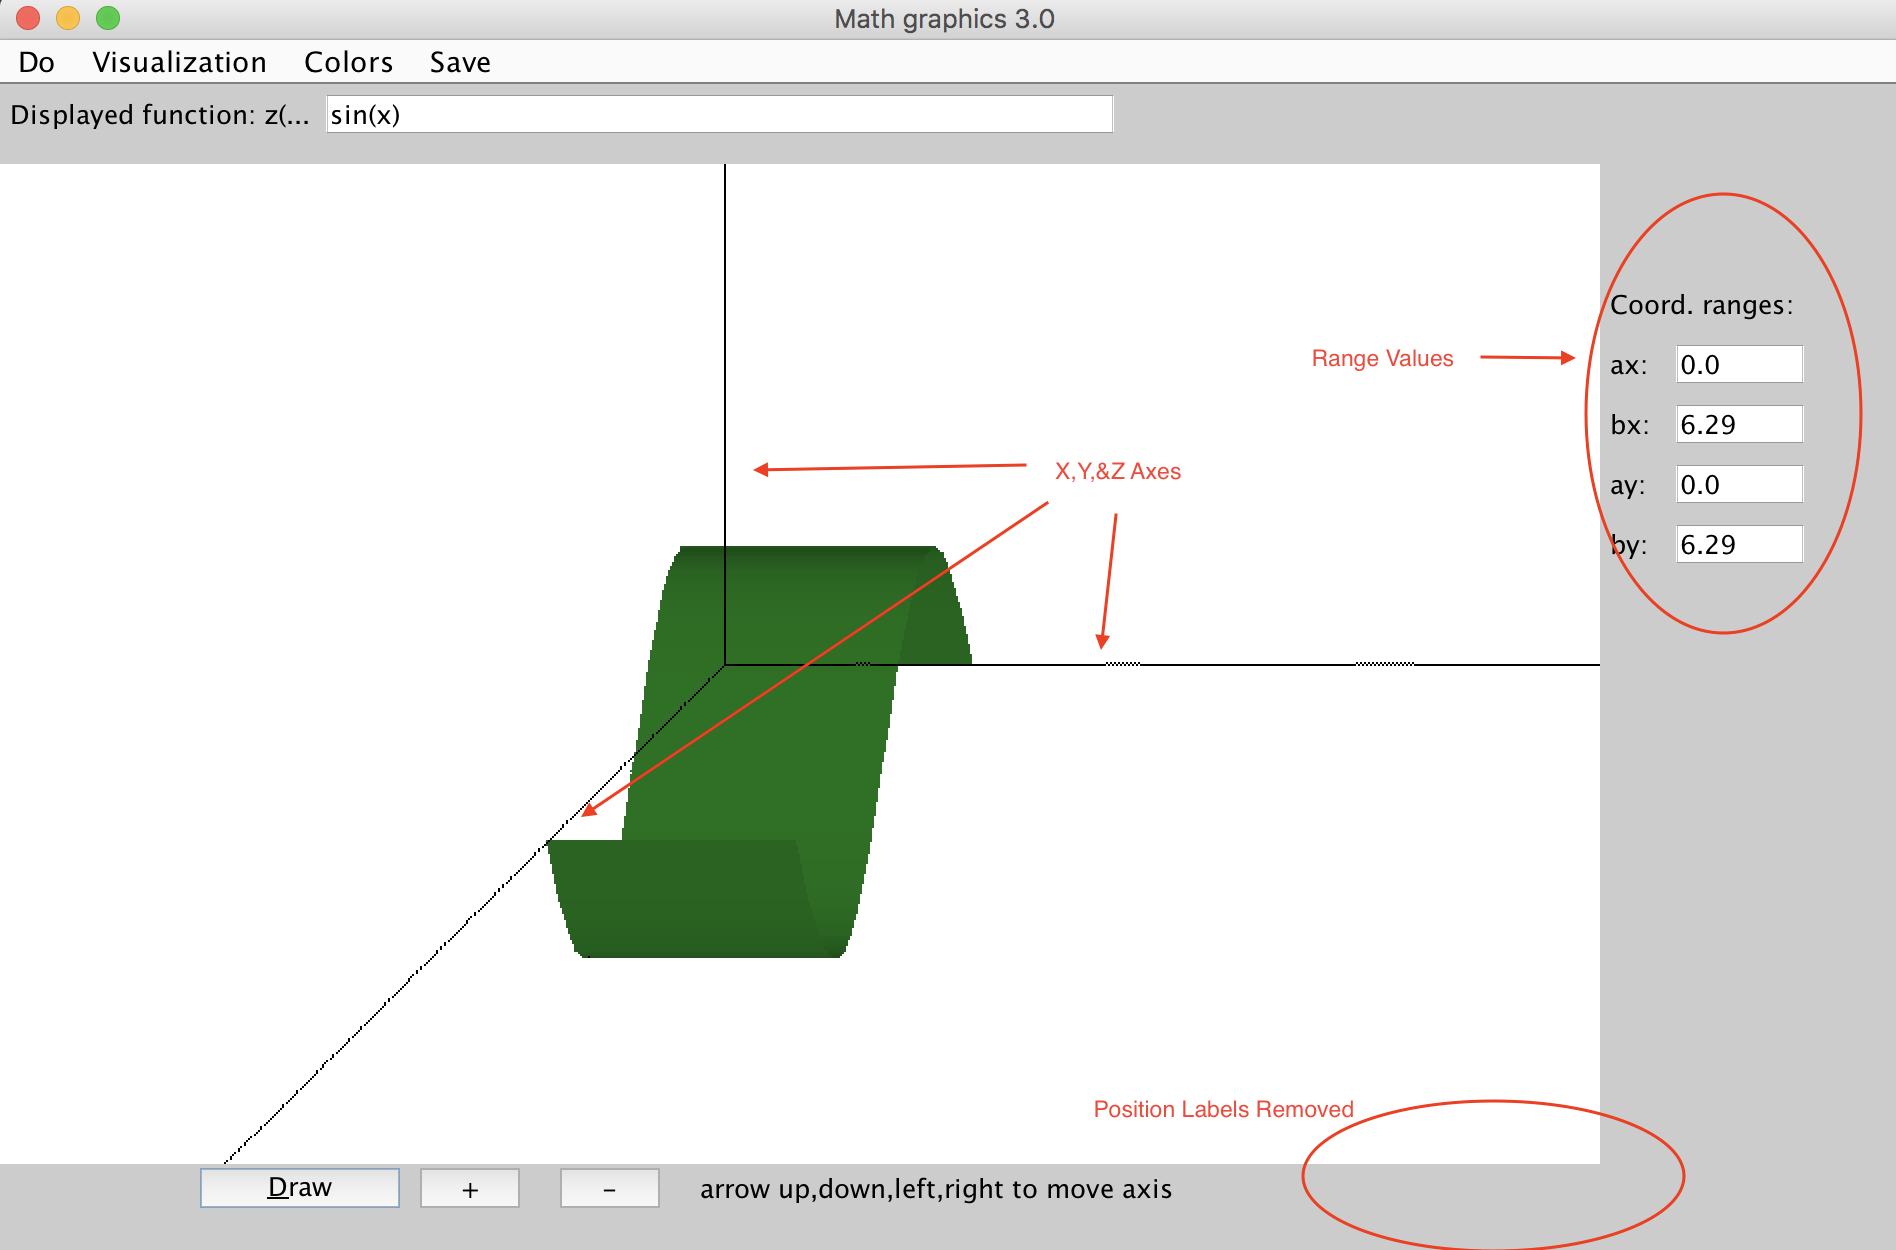
\includegraphics[scale=.35]{3DView}
			\caption{Cartesian 3D with changes to window annotated in red and $sin(x)$ function displayed}
			\end{figure}

		\section{User Configuration}
		\subsection{Changing Colors}
		Aside from performing complex mathematical functions, Math Grapher also gives the user the option to customize the appearance of the program. In order to do this the user can select the ``Colors'' drop-down menu followed by ``Choose Colors.'' 

		\subsubsection{Color Change Window}
		After the user has selected the appropriate menu items to change the colors, a pop-up window will appear. The pop-up window will reference a number of different parts of the program that can have the colors customized and changed. In this particular case, the reader can see that the background color of the graph is white, the panel color is gray, the line color of the function to be drawn is a dark blue, the derivative line is red, and the grid axis color is black. Not shown, the 3D rendering is an aquagreen color. Each available color has a respective ``More Colors'' button that, when selected, will open a traditional color palette tool from which the user can select which color they'd like. Once the color is selected, and ``Save'' is selected on the color panel pop-up window, the targeted color element will change. 
		\begin{figure}[h!]
		\centering
		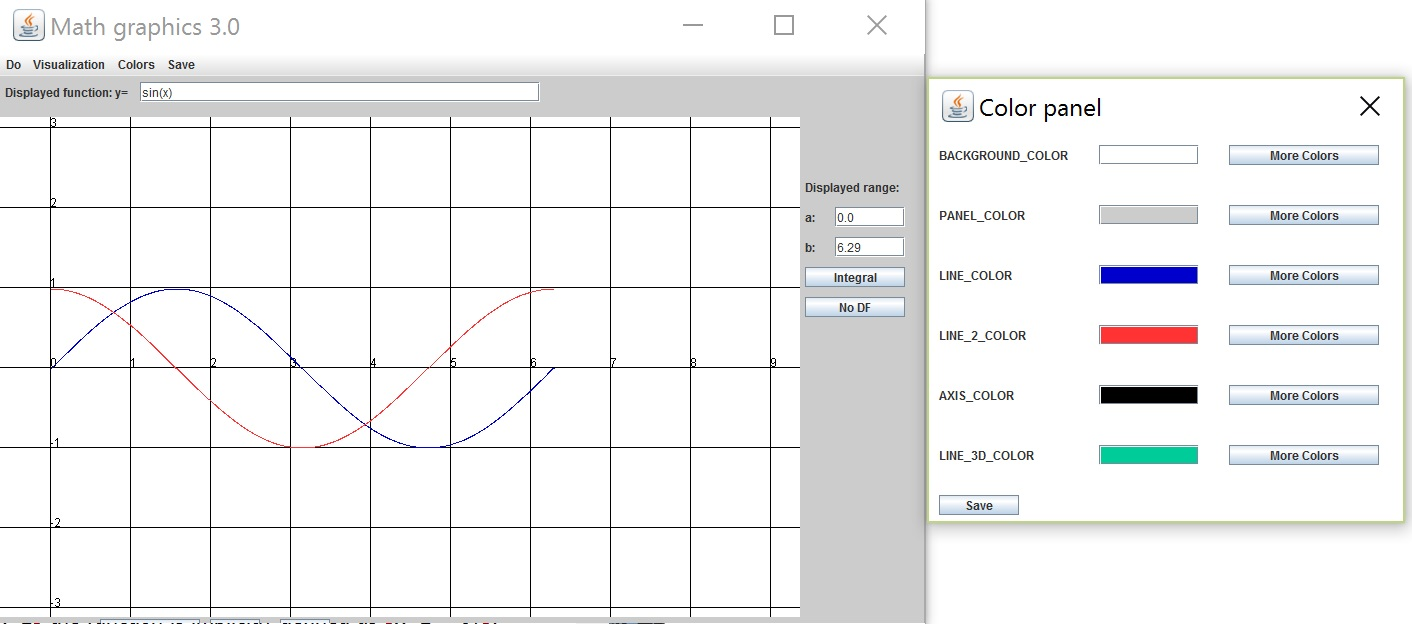
\includegraphics[scale =.70]{ColorPanel}
		\caption{The color panel window opens}
		\end{figure}
				 
		 \begin{figure}[h!]
		 \centering
		 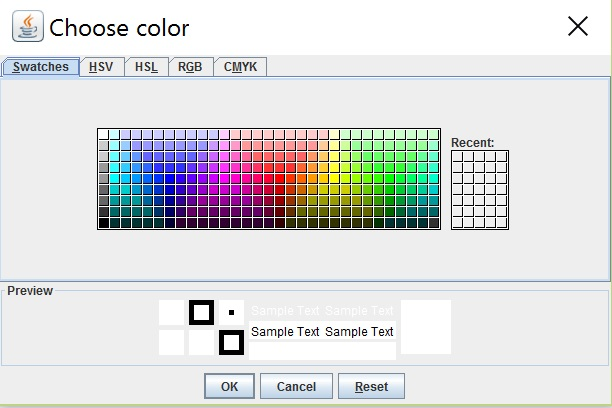
\includegraphics[scale=.70]{colorChooser}
		 \caption{The palette window opens when the ``More Colors'' button is clicked}
		 \end{figure}
		
		\pagebreak
		\section{Saving Files}
		 The output of the Math Grapher program can be sent to a file in two ways: as an image and as character separated values in a text file. 
		 \subsection{Image Saving}
		 Saving the image of the graph works in all 2D modes as well as in 3D. In order to save the image of the graph, simply select ``Save'' from the drop down menu followed by the selection of ``Save Image.'' The image must be saved as a jpg file. Thus, even if the user does not input the correct .jpg filename extension, Math Grapher will change the file to a .jpg file. 
		 \subsection{Save Data to Text File}
		 Another method to save data from Math Grapher is to output the data to a text file. To do this, select  ``Export Data'' from the drop down menu bar. After which, an export data panel pop-up window will appear. On this panel, when the user chooses ``Browse,'' they're then prompted to save their file. The file can only be saved as a .txt file. Thus, even if the user does not add the filename extension, it will be converted to a .txt file. The user also has the option to select how they'd like each value separated (comma, ampersand, etc...) and how they'd like each data entry separated (usually a new line character). 
\end {document}